% answers.tex —— 2018 年上海市春季高考数学试卷 · 参考答案与详细解析片段
% 由 tools/generate_projects.py 依来源总账自 2018/2018_数学真题_春季上海_试题.md + 2018/2018_数学真题_春季上海_解析正文.md + 2018/2018_数学真题_春季上海_答案要点.md 生成，勿手改（改源 MD 后重跑）


\begin{gktip}
以下解答以固定 PDF 第 1–6 页题面为准，不以第 7 页源载“参考答案”替代推导。来源发布者及源载答案的官方身份未核。Q17、Q18的文字缺项保留原样，相关推导只在明示假设下成立。Q21(3)按原卷第 6 页明确印出的“前 $n$ 项和”独立求解。
\end{gktip}

\begin{answer}
\gksolhead{1}{}

\textbf{题目}：

不等式 $|x|>1$ 的解集为 $\underline{\qquad}$。

\Needspace{4\baselineskip}
\textbf{解析}

$|x|>1$ 等价于 $x<-1$ 或 $x>1$，故解集为 $(-\infty,-1)\cup(1,+\infty)$。

\gkanswer{答案：$(-\infty,-1)\cup(1,+\infty)$}

\end{answer}
\begin{answer}
\gksolhead{2}{}

\textbf{题目}：

计算：$\displaystyle\lim_{n\to\infty}\frac{3n-1}{n+2}=\underline{\qquad}$。

\Needspace{4\baselineskip}
\textbf{解析}

\Needspace{5\baselineskip}
分子、分母同除以 $n$，得
\nopagebreak[4]
\[
\lim_{n\to\infty}\frac{3n-1}{n+2}
=\lim_{n\to\infty}\frac{3-1/n}{1+2/n}=3\text{。}
\]

\gkanswer{答案：$3$}

\end{answer}
\begin{answer}
\gksolhead{3}{}

\textbf{题目}：

设集合 $A=\{x\mid 0<x<2\}$，$B=\{x\mid -1<x<1\}$，则 $A\cap B=\underline{\qquad}$。

\Needspace{4\baselineskip}
\textbf{解析}

由 $A=(0,2)$、$B=(-1,1)$，可得 $A\cap B=(0,1)$。

\gkanswer{答案：$(0,1)$}

\end{answer}
\begin{answer}
\gksolhead{4}{}

\textbf{题目}：

若复数 $z=1+i$（$i$ 是虚数单位），则 $z+\dfrac{2}{z}=\underline{\qquad}$。

\Needspace{4\baselineskip}
\textbf{解析}

\nopagebreak[4]
\[
\frac2{1+i}=\frac{2(1-i)}{(1+i)(1-i)}=1-i\text{，}
\]
所以 $z+2/z=(1+i)+(1-i)=2$。

\gkanswer{答案：$2$}

\end{answer}
\begin{answer}
\gksolhead{5}{}

\textbf{题目}：

已知 $\{a_n\}$ 是等差数列，若 $a_2+a_8=10$，则 $a_3+a_5+a_7=\underline{\qquad}$。

\Needspace{4\baselineskip}
\textbf{解析}

等差数列中 $a_2+a_8=2a_5=10$，故 $a_5=5$；又 $a_3+a_7=2a_5=10$。因此 $a_3+a_5+a_7=15$。

\gkanswer{答案：$15$}

\end{answer}
\begin{answer}
\gksolhead{6}{}

\textbf{题目}：

已知平面上动点 $P$ 到两个定点 $(1,0)$ 和 $(-1,0)$ 的距离之和等于 $4$，则动点 $P$ 的轨迹方程为 $\underline{\qquad}$。

\Needspace{4\baselineskip}
\textbf{解析}

轨迹是以 $(1,0)$、$(-1,0)$ 为焦点的椭圆。焦点距离和为 $4$，故半长轴 $a=2$，半焦距 $c=1$，从而 $b^2=a^2-c^2=3$，轨迹方程为 $x^2/4+y^2/3=1$。

\gkanswer{答案：$\dfrac{x^2}{4}+\dfrac{y^2}{3}=1$}

\end{answer}
\begin{answer}
\gksolhead{7}{}

\textbf{题目}：

如图，在长方体 $ABCD-A_1B_1C_1D_1$ 中，$AB=3$，$BC=4$，$AA_1=5$，$O$ 是 $A_1C_1$ 的中点，则三棱锥 $A-A_1OB_1$ 的体积为 $\underline{\qquad}$。
\nopagebreak[4]
\begin{center}% Source: src-b19b233abb266d1b051ded3c332a399c1722d8192d07ce1bf2234dda57bd25bc, PDF p.1.
% Topology follows the source; oblique projection is schematic, not metric.
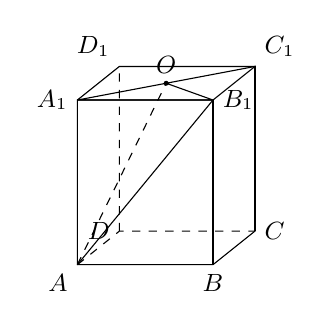
\begin{tikzpicture}[scale=0.82, every node/.style={font=\small}]
  \coordinate (A) at (0,0);
  \coordinate (B) at (2.1,0);
  \coordinate (C) at (2.75,0.52);
  \coordinate (D) at (0.65,0.52);
  \coordinate (A1) at (0,2.55);
  \coordinate (B1) at (2.1,2.55);
  \coordinate (C1) at (2.75,3.07);
  \coordinate (D1) at (0.65,3.07);
  \coordinate (O) at (1.375,2.81);
  \draw (A)--(B)--(C)--(C1)--(B1)--(A1)--cycle;
  \draw (C1)--(D1)--(A1);
  \draw[dashed] (A)--(D)--(C) (D)--(D1);
  \draw (A)--(A1) (B)--(B1) (C)--(C1);
  \draw (A1)--(C1) (A1)--(B1) (O)--(B1) (A)--(B1);
  \draw[dashed] (A)--(O);
  \fill (O) circle (1.1pt);
  \node[below left] at (A) {$A$};
  \node[below] at (B) {$B$};
  \node[right] at (C) {$C$};
  \node[left] at (D) {$D$};
  \node[left] at (A1) {$A_1$};
  \node[right] at (B1) {$B_1$};
  \node[above right] at (C1) {$C_1$};
  \node[above left] at (D1) {$D_1$};
  \node[above] at (O) {$O$};
\end{tikzpicture}
\end{center}
\nopagebreak[4]
\Needspace{4\baselineskip}
\textbf{解析}
\nopagebreak[4]
\begin{center}% Source: src-b19b233abb266d1b051ded3c332a399c1722d8192d07ce1bf2234dda57bd25bc, PDF p.1.
% Topology follows the source; oblique projection is schematic, not metric.
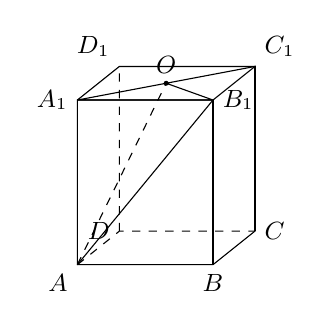
\begin{tikzpicture}[scale=0.82, every node/.style={font=\small}]
  \coordinate (A) at (0,0);
  \coordinate (B) at (2.1,0);
  \coordinate (C) at (2.75,0.52);
  \coordinate (D) at (0.65,0.52);
  \coordinate (A1) at (0,2.55);
  \coordinate (B1) at (2.1,2.55);
  \coordinate (C1) at (2.75,3.07);
  \coordinate (D1) at (0.65,3.07);
  \coordinate (O) at (1.375,2.81);
  \draw (A)--(B)--(C)--(C1)--(B1)--(A1)--cycle;
  \draw (C1)--(D1)--(A1);
  \draw[dashed] (A)--(D)--(C) (D)--(D1);
  \draw (A)--(A1) (B)--(B1) (C)--(C1);
  \draw (A1)--(C1) (A1)--(B1) (O)--(B1) (A)--(B1);
  \draw[dashed] (A)--(O);
  \fill (O) circle (1.1pt);
  \node[below left] at (A) {$A$};
  \node[below] at (B) {$B$};
  \node[right] at (C) {$C$};
  \node[left] at (D) {$D$};
  \node[left] at (A1) {$A_1$};
  \node[right] at (B1) {$B_1$};
  \node[above right] at (C1) {$C_1$};
  \node[above left] at (D1) {$D_1$};
  \node[above] at (O) {$O$};
\end{tikzpicture}
\end{center}
\nopagebreak[4]
取坐标 $A=(0,0,0)$、$B=(3,0,0)$、$C=(3,4,0)$、$A_1=(0,0,5)$、$B_1=(3,0,5)$、$C_1=(3,4,5)$。于是 $O=(3/2,2,5)$。三角形 $A_1OB_1$ 的底 $A_1B_1$ 长为 $3$，高为 $2$，面积为 $3$。点 $A$ 到平面 $A_1OB_1$ 的距离为 $5$，故三棱锥体积为 $\frac13\cdot3\cdot5=5$。

\gkanswer{答案：$5$}

\end{answer}
\begin{answer}
\gksolhead{8}{}

\textbf{题目}：

某校组队参加辩论赛，从 6 名学生中选出 4 人分别担任一、二、三、四辩，若其中学生甲必须参赛且不担任四辩，则不同的安排方法种数为 $\underline{\qquad}$（结果用数值表示）。

\Needspace{4\baselineskip}
\textbf{解析}

甲不能担任四辩，故甲有前三个辩位可选，共 $3$ 种。选定甲的位置后，其余三个位置从另外 $5$ 人中排列，方法数为 $5\cdot4\cdot3=60$。总数为 $3\cdot60=180$。

\gkanswer{答案：$180$}

\end{answer}
\begin{answer}
\gksolhead{9}{}

\textbf{题目}：

设 $a\in\mathbb R$，若 $\left(x^2+\dfrac{2}{x}\right)^9$ 与 $\left(x+\dfrac{a}{x^2}\right)^9$ 的二项展开式中的常数项相等，则 $a=\underline{\qquad}$。

\Needspace{4\baselineskip}
\textbf{解析}

在 $(x^2+2/x)^9$ 中，若取 $k$ 个 $2/x$，幂次为 $18-3k$；常数项对应 $k=6$，系数为 $\binom96 2^6=5376$。在 $(x+a/x^2)^9$ 中取 $k$ 个 $a/x^2$，幂次为 $9-3k$；常数项对应 $k=3$，系数为 $\binom93a^3=84a^3$。令二者相等，得 $a^3=64$，所以 $a=4$。

\gkanswer{答案：$4$}

\end{answer}
\begin{answer}
\gksolhead{10}{}

\textbf{题目}：

设 $m\in\mathbb R$，若 $z$ 是关于 $x$ 的方程 $x^2+mx+m^2-1=0$ 的一个虚根，则 $|z|$ 的取值范围是 $\underline{\qquad}$。

\Needspace{4\baselineskip}
\textbf{解析}

方程有虚根要求判别式 $m^2-4(m^2-1)=4-3m^2<0$，即 $m^2>4/3$。两根互为共轭，根模平方等于根的乘积 $m^2-1$，因此 $|z|=\sqrt{m^2-1}>1/\sqrt3$。当 $|m|$ 趋近 $2/\sqrt3$ 时模趋近 $1/\sqrt3$ 但不取到，故范围为 $(\sqrt3/3,+\infty)$。

\gkanswer{答案：$(\dfrac{\sqrt3}{3},+\infty)$}

\end{answer}
\begin{answer}
\gksolhead{11}{}

\textbf{题目}：

设 $a>0$，函数 $f(x)=x+2(1-x)\sin(ax)$，$x\in(0,1)$，若函数 $y=2x-1$ 与 $y=f(x)$ 的图像有且仅有两个不同的公共点，则 $a$ 的取值范围是 $\underline{\qquad}$。

\Needspace{4\baselineskip}
\textbf{解析}

\Needspace{5\baselineskip}
两图像相交满足
\nopagebreak[4]
\[
x+2(1-x)\sin(ax)=2x-1
\quad\Longleftrightarrow\quad
(1-x)(2\sin(ax)+1)=0\text{。}
\]
由于 $x\in(0,1)$，需 $\sin(ax)=-1/2$。正数解按递增次序为 $7\pi/6,11\pi/6,19\pi/6,\ldots$。恰有两个解落在 $0<ax<a$，等价于 $a>11\pi/6$ 且 $a\leq19\pi/6$。

\gkanswer{答案：$(\dfrac{11\pi}{6},\dfrac{19\pi}{6}]$}

\end{answer}
\begin{answer}
\gksolhead{12}{}

\textbf{题目}：

如图，正方形 $ABCD$ 的边长为 20 米，圆 $O$ 的半径为 1 米，圆心是正方形的中心，点 $P\text{、}Q$ 分别在线段 $AD\text{、}CB$ 上，若线段 $PQ$ 与圆 $O$ 有公共点，则称点 $Q$ 在点 $P$ 的“盲区”中，已知点 $P$ 以 1.5 米/秒的速度从 $A$ 出发向 $D$ 移动，同时，点 $Q$ 以 1 米/秒的速度从 $C$ 出发向 $B$ 移动，则在点 $P$ 从 $A$ 移动到 $D$ 的过程中，点 $Q$ 在点 $P$ 的盲区中的时长约为 $\underline{\qquad}$ 秒（精确到 0.1）。
\nopagebreak[4]
\begin{center}% Source: src-b19b233abb266d1b051ded3c332a399c1722d8192d07ce1bf2234dda57bd25bc, PDF p.1.
% Square, disk, and a segment joining the two opposite sides; schematic only.
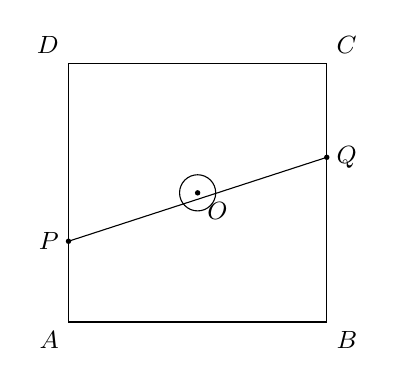
\begin{tikzpicture}[scale=0.82, every node/.style={font=\small}]
  \coordinate (A) at (0,0);
  \coordinate (B) at (4,0);
  \coordinate (C) at (4,4);
  \coordinate (D) at (0,4);
  \coordinate (O) at (2,2);
  \coordinate (P) at (0,1.25);
  \coordinate (Q) at (4,2.55);
  \draw (A)--(B)--(C)--(D)--cycle;
  \draw (O) circle[radius=0.28];
  \draw (P)--(Q);
  \fill (O) circle (1.2pt);
  \fill (P) circle (1.2pt);
  \fill (Q) circle (1.2pt);
  \node[below left] at (A) {$A$};
  \node[below right] at (B) {$B$};
  \node[above right] at (C) {$C$};
  \node[above left] at (D) {$D$};
  \node[below right] at (O) {$O$};
  \node[left] at (P) {$P$};
  \node[right] at (Q) {$Q$};
\end{tikzpicture}
\end{center}
\nopagebreak[4]
\Needspace{4\baselineskip}
\textbf{解析}
\nopagebreak[4]
\begin{center}% Source: src-b19b233abb266d1b051ded3c332a399c1722d8192d07ce1bf2234dda57bd25bc, PDF p.1.
% Square, disk, and a segment joining the two opposite sides; schematic only.
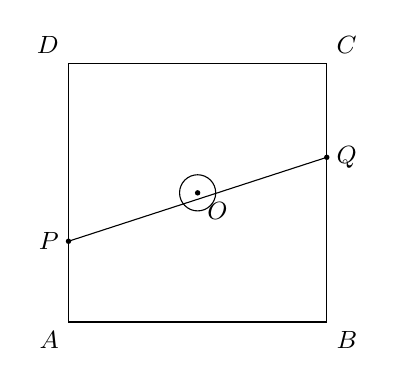
\begin{tikzpicture}[scale=0.82, every node/.style={font=\small}]
  \coordinate (A) at (0,0);
  \coordinate (B) at (4,0);
  \coordinate (C) at (4,4);
  \coordinate (D) at (0,4);
  \coordinate (O) at (2,2);
  \coordinate (P) at (0,1.25);
  \coordinate (Q) at (4,2.55);
  \draw (A)--(B)--(C)--(D)--cycle;
  \draw (O) circle[radius=0.28];
  \draw (P)--(Q);
  \fill (O) circle (1.2pt);
  \fill (P) circle (1.2pt);
  \fill (Q) circle (1.2pt);
  \node[below left] at (A) {$A$};
  \node[below right] at (B) {$B$};
  \node[above right] at (C) {$C$};
  \node[above left] at (D) {$D$};
  \node[below right] at (O) {$O$};
  \node[left] at (P) {$P$};
  \node[right] at (Q) {$Q$};
\end{tikzpicture}
\end{center}
\nopagebreak[4]
\Needspace{5\baselineskip}
按图设正方形坐标为 $A=(0,0)$、$D=(0,20)$、$C=(20,20)$、$B=(20,0)$，时间为 $t$ 秒，则 $P=(0,1.5t)$、$Q=(20,20-t)$，圆心 $O=(10,10)$。直线 $PQ$ 可写为
\nopagebreak[4]
\[
(20-2.5t)x-20y+30t=0\text{。}
\]
\Needspace{5\baselineskip}
圆心到该直线的距离为 $\dfrac{5t}{\sqrt{(20-2.5t)^2+400}}$。令距离不大于圆半径 $1$，得
\nopagebreak[4]
\[
3t^2+16t-128\leq0\text{。}
\]
非负时间解为 $0\leq t\leq\dfrac83(\sqrt7-1)\approx4.3887$。在该区间内垂足落在线段 $PQ$ 上，故盲区时长约为 $4.4$ 秒。水平运动坐标会与源图的 $AD$、$CB$ 方向不符，不能据此计算。

\gkanswer{答案：约 $4.4$ 秒}

\end{answer}
\begin{answer}
\gksolhead{13}{}

\textbf{题目}：

下列函数中，为偶函数的是\mbox{（　　）}。

（A）$y=x^{-2}$　　（B）$y=x^{1/3}$　　（C）$y=x^{-1/2}$　　（D）$y=x^3$

\Needspace{4\baselineskip}
\textbf{解析}

$y=x^{-2}$ 的定义域为 $\mathbb R\setminus\{0\}$，关于原点对称，且 $f(-x)=(-x)^{-2}=x^{-2}=f(x)$，所以它是偶函数，选 A。

\gkanswer{答案：A}

\end{answer}
\begin{answer}
\gksolhead{14}{}

\textbf{题目}：

如图，在直三棱柱 $ABC-A_1B_1C_1$ 的棱所在的直线中，与直线 $BC_1$ 异面的直线的条数为\mbox{（　　）}。

（A）1　　（B）2　　（C）3　　（D）4
\nopagebreak[4]
\begin{center}% Source: src-b19b233abb266d1b051ded3c332a399c1722d8192d07ce1bf2234dda57bd25bc, PDF p.2.
% Right triangular prism topology and the specified line BC_1; schematic projection.
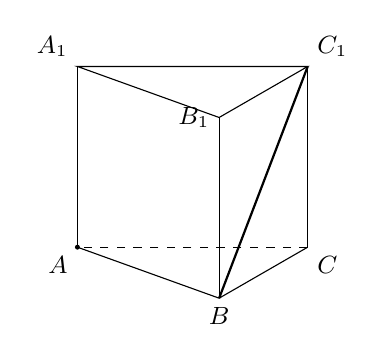
\begin{tikzpicture}[scale=0.9, every node/.style={font=\small}]
  \coordinate (A) at (0,0);
  \coordinate (B) at (2.0,-0.72);
  \coordinate (C) at (3.25,0);
  \coordinate (A1) at (0,2.55);
  \coordinate (B1) at (2.0,1.83);
  \coordinate (C1) at (3.25,2.55);
  \draw (A)--(B)--(C);
  \draw[dashed] (C)--(A);
  \draw (A1)--(B1)--(C1)--cycle;
  \draw (A)--(A1) (B)--(B1) (C)--(C1);
  \draw[thick] (B)--(C1);
  \fill (A) circle (1pt);
  \node[below left] at (A) {$A$};
  \node[below] at (B) {$B$};
  \node[below right] at (C) {$C$};
  \node[above left] at (A1) {$A_1$};
  \node[left] at (B1) {$B_1$};
  \node[above right] at (C1) {$C_1$};
\end{tikzpicture}
\end{center}
\nopagebreak[4]
\Needspace{4\baselineskip}
\textbf{解析}
\nopagebreak[4]
\begin{center}% Source: src-b19b233abb266d1b051ded3c332a399c1722d8192d07ce1bf2234dda57bd25bc, PDF p.2.
% Right triangular prism topology and the specified line BC_1; schematic projection.
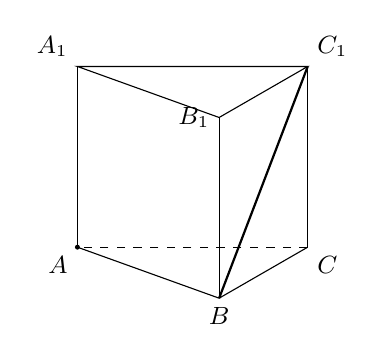
\begin{tikzpicture}[scale=0.9, every node/.style={font=\small}]
  \coordinate (A) at (0,0);
  \coordinate (B) at (2.0,-0.72);
  \coordinate (C) at (3.25,0);
  \coordinate (A1) at (0,2.55);
  \coordinate (B1) at (2.0,1.83);
  \coordinate (C1) at (3.25,2.55);
  \draw (A)--(B)--(C);
  \draw[dashed] (C)--(A);
  \draw (A1)--(B1)--(C1)--cycle;
  \draw (A)--(A1) (B)--(B1) (C)--(C1);
  \draw[thick] (B)--(C1);
  \fill (A) circle (1pt);
  \node[below left] at (A) {$A$};
  \node[below] at (B) {$B$};
  \node[below right] at (C) {$C$};
  \node[above left] at (A1) {$A_1$};
  \node[left] at (B1) {$B_1$};
  \node[above right] at (C1) {$C_1$};
\end{tikzpicture}
\end{center}
\nopagebreak[4]
三棱柱有九条棱所在直线。与 $BC_1$ 相交的六条是过 $B$ 的 $AB,BC,BB_1$ 与过 $C_1$ 的 $A_1C_1,B_1C_1,CC_1$。其余 $AC,A_1B_1,AA_1$ 均不与 $BC_1$ 相交且不平行，故为异面直线，共 $3$ 条，选 C。

\gkanswer{答案：C}

\end{answer}
\begin{answer}
\gksolhead{15}{}

\textbf{题目}：

设 $S_n$ 为数列 $\{a_n\}$ 的前 $n$ 项，“$\{a_n\}$ 是递增数列”是“$\{S_n\}$ 是递增数列”的\mbox{（　　）}。

（A）充分非必要条件　　（B）必要非充分条件

（C）充要条件　　（D）既非充分又非必要条件

\Needspace{4\baselineskip}
\textbf{解析}

$\{S_n\}$ 递增等价于每个 $a_n=S_n-S_{n-1}>0$（令 $S_0=0$）。这不推出 $\{a_n\}$ 递增，例如可取正但先大后小的数列。反过来，$\{a_n\}$ 递增也不保证每项为正，例如 $a_n=n-2$ 递增而首项为负。因此两命题互不推出，选 D。

\gkanswer{答案：D}

\end{answer}
\begin{answer}
\gksolhead{16}{}

\textbf{题目}：

已知 $A\text{、}B$ 为平面上的两个定点，且 $|\overrightarrow{AB}|=2$，该平面上的动线段 $PQ$ 的端点 $P\text{、}Q$，满足 $|\overrightarrow{AP}|\leq 5$，$\overrightarrow{AP}\cdot\overrightarrow{AB}=6$，$\overrightarrow{AQ}=-2\overrightarrow{AP}$，则动线段 $PQ$ 所形成图形的面积为\mbox{（　　）}。

（A）36　　（B）60　　（C）72　　（D）108

\Needspace{4\baselineskip}
\textbf{解析}

\Needspace{5\baselineskip}
令 $\overrightarrow{AB}$ 为横轴方向。由 $|\overrightarrow{AB}|=2$ 与 $\overrightarrow{AP}\cdot\overrightarrow{AB}=6$，可设 $\overrightarrow{AP}=(3,y)$。条件 $|\overrightarrow{AP}|\leq5$ 给出 $-4\leq y\leq4$。又 $\overrightarrow{AQ}=-2\overrightarrow{AP}$，线段 $PQ$ 上的点可写成 $t(3,y)$，其中 $-2\leq t\leq1$。参数映射 $(t,y)\mapsto(3t,ty)$ 的面积因子为 $3|t|$，故所成图形面积为
\nopagebreak[4]
\[
\int_{-2}^{1}\int_{-4}^{4}3|t|\,dy\,dt=60\text{，}
\]
选 B。

\gkanswer{答案：B（面积为 $60$）}

\end{answer}
\begin{answer}
\gksolhead{17}{}

\textbf{题目}：

已知 $y=\cos x$。

（1） 若 $f(\alpha)=\dfrac13$，且 $\alpha\in[0,\pi]$，求 $f\left(\alpha-\dfrac\pi3\right)$ 的值；

（2） 求函数 $y=f(2x)-2f(x)$ 的最小值。

\begin{gktip}
原文未见 $f$ 的显式定义；此处保持“已知 $y=\cos x$”原文，不补为 $f(x)=\cos x$。
\end{gktip}

\Needspace{4\baselineskip}
\textbf{解析}

\Needspace{4\baselineskip}
\textbf{解析}

原文只写“已知 $y=\cos x$”，后文却使用 $f$，未显式定义 $f$。以下仅在另加假设 $f(x)=\cos x$ 时成立。由 $\cos\alpha=1/3$ 且 $\alpha\in[0,\pi]$，得 $\sin\alpha=2\sqrt2/3$。于是

\gksubpart{(1) 条件推导}

\nopagebreak[4]
\[
f\left(\alpha-\frac\pi3\right)
=\cos\left(\alpha-\frac\pi3\right)
=\frac16+\frac{\sqrt6}{3}
=\frac{1+2\sqrt6}{6}\text{。}
\]

\gksubpart{(2) 条件推导}

令 $u=\cos x\in[-1,1]$，则 $f(2x)-2f(x)=2u^2-2u-1$，其在 $u=1/2$ 处取最小值 $-3/2$。原文缺少 $f$ 的定义，因此两问正式答案仍为 U/PENDING；以上不据源载答案页补字。

\gkanswer{答案（1）：U/PENDING；若原意为 $f(x)=\cos x$，则条件结果为 $\dfrac{1+2\sqrt6}{6}$。}

\gkanswer{答案（2）：U/PENDING；若原意为 $f(x)=\cos x$，则条件结果为 $-\dfrac32$。}

\end{answer}
\begin{answer}
\gksolhead{18}{}

\textbf{题目}：

已知 $a\in\mathbb R$，双曲线 $\Gamma:\dfrac{x^2}{a^2}-y^2=1$。

（1） 若点 $(2,1)$ 在上，求 $\Gamma$ 的焦点坐标；

（2） 若 $a=1$，直线 $y=kx+1$ 与 $\Gamma$ 相交于 $A\text{、}B$ 两点，且线段 $AB$ 中点的横坐标为 1，求实数 $k$ 的值。

\begin{gktip}
原文“若点 $(2,1)$ 在上”未在“在上”之间标出曲线名称；此处照录，不补入 $\Gamma$。
\end{gktip}

\Needspace{4\baselineskip}
\textbf{解析}

\gksubpart{(1) 条件推导}

原文称点 $(2,1)$“在上”，没有写明曲线名称。若补充条件 $(2,1)\in\Gamma$，则 $4/a^2-1=1$，从而 $a^2=2$。双曲线焦点为 $(\pm\sqrt{a^2+1},0)$，即 $(\sqrt3,0)$、$(-\sqrt3,0)$。该归属关系未由现有题面确定，故正式答案为 U/PENDING。

\gksubpart{(2)}

\Needspace{5\baselineskip}
取 $a=1$，将 $y=kx+1$ 代入 $x^2-y^2=1$，得
\nopagebreak[4]
\[
(1-k^2)x^2-2kx-2=0\text{。}
\]
两交点横坐标的平均数为 $k/(1-k^2)$。令其等于 $1$，得 $k^2+k-1=0$。所对应的根中，$k=(\sqrt5-1)/2$ 满足相交于两个不同实点的条件；另一个根不满足该条件，故 $k=(\sqrt5-1)/2$。

\gkanswer{答案（1）：U/PENDING；若 $(2,1)\in\Gamma$，则焦点为 $(\sqrt3,0)$、$(-\sqrt3,0)$。}

\gkanswer{答案（2）：$k=\dfrac{\sqrt5-1}{2}$}

\end{answer}
\begin{answer}
\gksolhead{19}{}

\textbf{题目}：

利用“平行于圆锥母线的平面截圆锥面，所得截线是抛物线”的几何原理，某快餐店用两个射灯（射出的光锥为圆锥）在广告牌上投影出某标识，如图1所示，图2是投影射出的抛物线的平面图，图3是一个射灯投影的直观图，在图2与图3中，点 $O\text{、}A\text{、}B$ 在抛物线上，$OC$ 是抛物线的对称轴，$OC\perp AB$ 于 $C$，$AB=3$ 米，$OC=4.5$ 米。

（1） 求抛物线的焦点到准线的距离；

（2） 在图3中，已知 $OC$ 平行于圆锥的母线 $SD$，$AB\text{、}DE$ 是圆锥底面的直径，求圆锥的母线与轴的夹角大小（精确到 $0.01^\circ$）。
\nopagebreak[4]
\begin{center}% Source: src-b19b233abb266d1b051ded3c332a399c1722d8192d07ce1bf2234dda57bd25bc, PDF p.4.
% Include the source-context photograph as a raster asset; mathematical diagrams are redrawn separately.
\begin{center}
  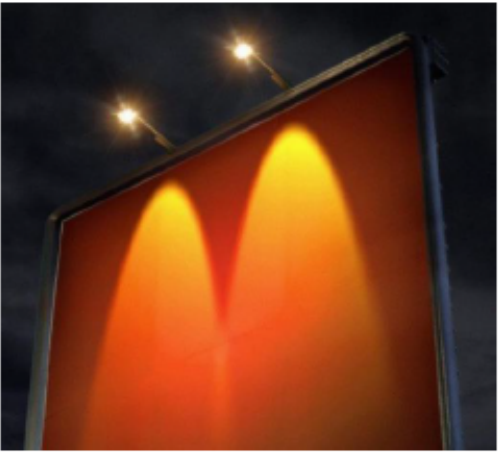
\includegraphics[width=0.46\linewidth]{assets/f2018_shanghai_spring_q19_photo.png}
\end{center}
\end{center}
\nopagebreak[4]
\nopagebreak[4]
\begin{center}% Source: src-b19b233abb266d1b051ded3c332a399c1722d8192d07ce1bf2234dda57bd25bc, PDF p.4.
% Reproduces the labeled parabola relation; curve shape and offset context are schematic.
\begin{tikzpicture}[scale=0.82, every node/.style={font=\small}]
  \coordinate (O) at (0,2.8);
  \coordinate (A) at (-1.2,0);
  \coordinate (B) at (1.2,0);
  \coordinate (C) at (0,0);
  \draw[densely dashed, domain=-2.55:-1.25, samples=60, variable=\x]
    plot (\x,{2.8-1.95*(\x+1.25)^2});
  \draw[thick, domain=-1.2:1.2, samples=80, variable=\x]
    plot (\x,{2.8-1.95*\x^2});
  \draw (A)--(B);
  \draw (O)--(C);
  \draw (0,0.18)--(0.18,0.18)--(0.18,0);
  \fill (O) circle (1pt);
  \fill (A) circle (1pt);
  \fill (B) circle (1pt);
  \node[above] at (O) {$O$};
  \node[below left] at (A) {$A$};
  \node[below right] at (B) {$B$};
  \node[below right] at (C) {$C$};
\end{tikzpicture}
\end{center}
\nopagebreak[4]
\nopagebreak[4]
\begin{center}% Source: src-b19b233abb266d1b051ded3c332a399c1722d8192d07ce1bf2234dda57bd25bc, PDF p.4.
% Cone topology and parallel OC/SD relation; projection is schematic, not metric.
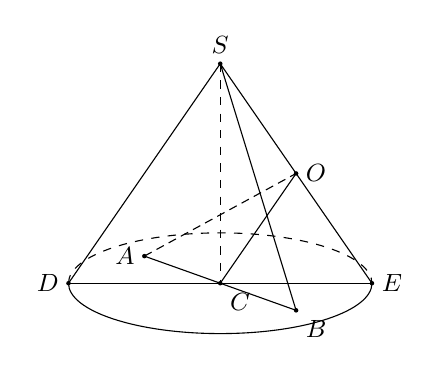
\begin{tikzpicture}[scale=0.82, every node/.style={font=\small}]
  \coordinate (S) at (0,3.4);
  \coordinate (D) at (-2.35,0);
  \coordinate (E) at (2.35,0);
  \coordinate (C) at (0,0);
  \coordinate (A) at (-1.175,0.42);
  \coordinate (B) at (1.175,-0.42);
  \coordinate (O) at (1.175,1.7);
  \draw (S)--(D) (S)--(E) (S)--(B);
  \draw[dashed] (S)--(C);
  \draw (D) arc[start angle=180,end angle=360,x radius=2.35,y radius=0.78];
  \draw[dashed] (D) arc[start angle=180,end angle=0,x radius=2.35,y radius=0.78];
  \draw (D)--(E);
  \draw (A)--(B);
  \draw (C)--(O);
  \draw[densely dashed] (A)--(O);
  \fill (S) circle (1pt);
  \fill (D) circle (1pt);
  \fill (E) circle (1pt);
  \fill (A) circle (1pt);
  \fill (B) circle (1pt);
  \fill (C) circle (1pt);
  \fill (O) circle (1pt);
  \node[above] at (S) {$S$};
  \node[left] at (D) {$D$};
  \node[right] at (E) {$E$};
  \node[left] at (A) {$A$};
  \node[below right] at (B) {$B$};
  \node[below right] at (C) {$C$};
  \node[right] at (O) {$O$};
\end{tikzpicture}
\end{center}
\nopagebreak[4]
\Needspace{4\baselineskip}
\textbf{解析}
\nopagebreak[4]
\begin{center}% Source: src-b19b233abb266d1b051ded3c332a399c1722d8192d07ce1bf2234dda57bd25bc, PDF p.4.
% Reproduces the labeled parabola relation; curve shape and offset context are schematic.
\begin{tikzpicture}[scale=0.82, every node/.style={font=\small}]
  \coordinate (O) at (0,2.8);
  \coordinate (A) at (-1.2,0);
  \coordinate (B) at (1.2,0);
  \coordinate (C) at (0,0);
  \draw[densely dashed, domain=-2.55:-1.25, samples=60, variable=\x]
    plot (\x,{2.8-1.95*(\x+1.25)^2});
  \draw[thick, domain=-1.2:1.2, samples=80, variable=\x]
    plot (\x,{2.8-1.95*\x^2});
  \draw (A)--(B);
  \draw (O)--(C);
  \draw (0,0.18)--(0.18,0.18)--(0.18,0);
  \fill (O) circle (1pt);
  \fill (A) circle (1pt);
  \fill (B) circle (1pt);
  \node[above] at (O) {$O$};
  \node[below left] at (A) {$A$};
  \node[below right] at (B) {$B$};
  \node[below right] at (C) {$C$};
\end{tikzpicture}
\end{center}
\nopagebreak[4]
\nopagebreak[4]
\begin{center}% Source: src-b19b233abb266d1b051ded3c332a399c1722d8192d07ce1bf2234dda57bd25bc, PDF p.4.
% Cone topology and parallel OC/SD relation; projection is schematic, not metric.
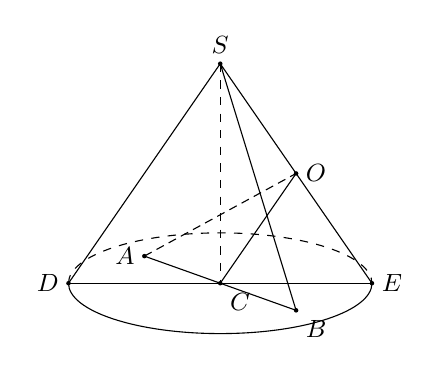
\begin{tikzpicture}[scale=0.82, every node/.style={font=\small}]
  \coordinate (S) at (0,3.4);
  \coordinate (D) at (-2.35,0);
  \coordinate (E) at (2.35,0);
  \coordinate (C) at (0,0);
  \coordinate (A) at (-1.175,0.42);
  \coordinate (B) at (1.175,-0.42);
  \coordinate (O) at (1.175,1.7);
  \draw (S)--(D) (S)--(E) (S)--(B);
  \draw[dashed] (S)--(C);
  \draw (D) arc[start angle=180,end angle=360,x radius=2.35,y radius=0.78];
  \draw[dashed] (D) arc[start angle=180,end angle=0,x radius=2.35,y radius=0.78];
  \draw (D)--(E);
  \draw (A)--(B);
  \draw (C)--(O);
  \draw[densely dashed] (A)--(O);
  \fill (S) circle (1pt);
  \fill (D) circle (1pt);
  \fill (E) circle (1pt);
  \fill (A) circle (1pt);
  \fill (B) circle (1pt);
  \fill (C) circle (1pt);
  \fill (O) circle (1pt);
  \node[above] at (S) {$S$};
  \node[left] at (D) {$D$};
  \node[right] at (E) {$E$};
  \node[left] at (A) {$A$};
  \node[below right] at (B) {$B$};
  \node[below right] at (C) {$C$};
  \node[right] at (O) {$O$};
\end{tikzpicture}
\end{center}
\nopagebreak[4]
\gksubpart{(1)}

以抛物线顶点 $O$ 为原点、对称轴为纵轴。弦 $AB=3$ 位于距顶点 $OC=4.5$ 的位置，故弦端点横坐标为 $\pm1.5$。设抛物线为 $x^2=4py$，代入 $(1.5,4.5)$ 得 $p=1/8$。焦点到准线的距离为 $2p=1/4$ 米。

\gksubpart{(2)}

圆锥底面直径 $AB=3$，半径为 $1.5$。在轴截面三角形 $SDE$ 中，$C$ 为 $DE$ 中点，且 $CO\parallel SD$；由中位线定理，$O$ 是 $SE$ 中点并有 $CO=SD/2$。已知 $CO=4.5$，故母线长 $SD=9$。若母线与轴的夹角为 $\theta$，轴截面中 $\sin\theta=1.5/9=1/6$，所以 $\theta=\arcsin(1/6)\approx9.59^\circ$。

\gkanswer{答案（1）：$\dfrac14$ 米}

\gkanswer{答案（2）：$\arcsin\dfrac16\approx9.59^\circ$}

\end{answer}
\begin{answer}
\gksolhead{20}{}

\textbf{题目}：

设 $a>0$，函数 $f(x)=\dfrac{1}{1+a\cdot2^x}$。

（1） 若 $a=1$，求 $f(x)$ 的反函数 $f^{-1}(x)$；

（2） 求函数 $y=f(x)\cdot f(-x)$ 的最大值（用 $a$ 表示）；

（3） 设 $g(x)=f(x)-f(x-1)$，若对任意 $x\in(-\infty,0]$，$g(x)\geq g(0)$ 恒成立，求 $a$ 取值范围。

\Needspace{4\baselineskip}
\textbf{解析}

\gksubpart{(1)}

当 $a=1$ 时，$y=1/(1+2^x)$，所以 $2^x=(1-y)/y$，得到反函数 $f^{-1}(x)=\log_2((1-x)/x)$，定义域为 $0<x<1$。

\gksubpart{(2)}

\nopagebreak[4]
\[
f(x)f(-x)=\frac1{1+a^2+a(2^x+2^{-x})}\text{。}
\]
由 $2^x+2^{-x}\geq2$，分母在 $x=0$ 时最小，最大值为 $1/(1+a)^2$。

\gksubpart{(3)}

\Needspace{5\baselineskip}
令 $t=2^x\in(0,1]$，则
\nopagebreak[4]
\[
g(x)=-h(t),\qquad
h(t)=\frac{at/2}{(1+at)(1+at/2)}\text{。}
\]
$h'(t)$ 的符号由 $1-a^2t^2/2$ 决定。若 $0<a\leq\sqrt2$，则 $h$ 在 $(0,1]$ 上递增，因而 $h(t)\leq h(1)$，即 $g(x)\geq g(0)$。若 $a>\sqrt2$，$h$ 在 $t=\sqrt2/a<1$ 处达到大于 $h(1)$ 的内部最大值，条件不成立。因此 $0<a\leq\sqrt2$。

\gkanswer{答案（1）：$f^{-1}(x)=\log_2\dfrac{1-x}{x}\quad(0<x<1)$}

\gkanswer{答案（2）：$\dfrac{1}{(1+a)^2}$，在 $x=0$ 处取到。}

\gkanswer{答案（3）：$0<a\leq\sqrt2$}

\end{answer}
\begin{answer}
\gksolhead{21}{}

\textbf{题目}：

\Needspace{5\baselineskip}
若 $\{c_n\}$ 是递增数列，数列 $\{a_n\}$ 满足：对任意 $n\in\mathbb N^*$，存在 $m\in\mathbb N^*$，使得
\nopagebreak[4]
\[
\frac{a_m-c_n}{a_m-c_{n+1}}\leq0,
\]
则称 $\{a_n\}$ 是 $\{c_n\}$ 的“分隔数列”。

（1） 设 $c_n=2n$，$a_n=n+1$，证明：数列 $\{a_n\}$ 是 $\{c_n\}$ 的分隔数列；

（2） 设 $c_n=n-4$，$S_n$ 是 $\{c_n\}$ 的前 $n$ 项和，$d_n=c_{3n-2}$，判断数列 $\{S_n\}$ 是否是数列 $\{d_n\}$ 的分隔数列，并说明理由；

（3） 设 $c_n=aq^{n-1}$，$T_n$ 是 $\{c_n\}$ 的前 $n$ 项和，若数列 $\{T_n\}$ 是 $\{c_n\}$ 的分隔数列，求实数 $a\text{、}q$ 的取值范围。

\begin{gktip}
原卷第 6 页明确印有“前 $n$ 项和”；此前转录漏掉“和”字，现已按原页更正。
\end{gktip}

\Needspace{4\baselineskip}
\textbf{解析}

不等式中的分母不得为零；对严格递增的 $\{c_n\}$，分式不大于零等价于 $c_n\leq a_m<c_{n+1}$。

\gksubpart{(1)}

对任意 $n$ 取 $m=2n-1$，则 $a_m=m+1=2n=c_n$，所给分式等于 $0$，故满足分隔数列定义。

\gksubpart{(2)}

由 $c_n=n-4$ 得 $S_n=n(n-7)/2$，又 $d_n=c_{3n-2}=3n-6$。取 $n=4$，需要某项 $S_m$ 落在 $[d_4,d_5)=[6,9)$。但 $m\leq7$ 时 $S_m\leq0$，$S_8=4$，而 $m\geq9$ 时 $S_m\geq9$，故不存在这样的 $m$，所以不是分隔数列。

\gksubpart{(3)}

\Needspace{5\baselineskip}
按原卷定义 $T_n=\sum_{j=1}^n c_j$。结合题首 $\{c_n\}$ 严格递增，对几何数列须有 $a>0$、$q>1$。此时
\nopagebreak[4]
\[
\frac{T_n}{c_{n+1}}=\frac{1-q^{-n}}{q-1}\text{。}
\]
对每个 $n$，$T_n\geq c_n$；分隔条件等价于 $T_n<c_{n+1}$。上式对所有 $n\geq1$ 严格小于 $1$ 当且仅当 $q\geq2$。因此 $a>0,q\geq2$。题面的“前 $n$ 项和”定义明确，答案不需要额外假设。

\gkanswer{答案（1）：见解析版}

\gkanswer{答案（2）：不是；取 $n=4$ 时不存在满足条件的 $m$。}

\gkanswer{答案（3）：$a>0,\ q\geq2$。}

\end{answer}